% !TeX root = ./thesis.tex
% !TeX spellcheck = hu_HU
% !TeX encoding = UTF-8
% !TeX program = pdflatex
% !TeX TXS-program:compile = txs:///python//usr/bin/python3
\documentclass[12pt,a4paper,oneside]{report}             % Egyoldalas (javasolt)
%\documentclass[11pt,a4paper,twoside,openright]{report}  % Duplex
% thanks to http://tex.stackexchange.com/a/47579/71109
\usepackage{pdfpages} 
\usepackage{ifxetex}
\usepackage{ifluatex}
\newif\ifxetexorluatex % a new conditional starts as false
\ifnum 0\ifxetex 1\fi\ifluatex 1\fi>0
   \xetexorluatextrue
\fi

\ifxetexorluatex
  \usepackage{fontspec}
\else
  \usepackage[T1]{fontenc}
  \usepackage[utf8]{inputenc}
  \usepackage[lighttt]{lmodern}
\fi

\usepackage[english,magyar]{babel} % Alapértelmezés szerint utoljára definiált nyelv lesz aktív, de később külön beállítjuk az aktív nyelvet.

%\usepackage{cmap}
\usepackage{amsfonts,amsmath,amssymb} % Mathematical symbols.
%\usepackage[ruled,boxed,resetcount,linesnumbered]{algorithm2e} % For pseudocodes. % beware: this is not compatible with LuaLaTeX, see http://tex.stackexchange.com/questions/34814/lualatex-and-algorithm2e
\usepackage{booktabs} % For publication quality tables for LaTeX
\usepackage{graphicx}

%\usepackage{fancyhdr}
%\usepackage{lastpage}

\usepackage{anysize}
%\usepackage{sectsty}
\usepackage{setspace} % For setting line spacing

\usepackage[unicode]{hyperref} % For hyperlinks in the generated document.
\usepackage{xcolor}
\usepackage{listings} % For source code snippets.

\usepackage[amsmath,thmmarks]{ntheorem} % Theorem-like environments.

\usepackage[hang]{caption}

\usepackage[list=true]{subcaption}	%tof url
\usepackage{tocloft}

\usepackage{datetime2}


\singlespacing

\newcommand{\selecthungarian}{
	\selectlanguage{magyar}
	\setlength{\parindent}{2em}
	\setlength{\parskip}{0em}
	\frenchspacing
}

\newcommand{\selectenglish}{
	\selectlanguage{english}
	\setlength{\parindent}{0em}
	\setlength{\parskip}{0.5em}
	\nonfrenchspacing
	\renewcommand{\figureautorefname}{Figure}
	\renewcommand{\tableautorefname}{Table}
	\renewcommand{\partautorefname}{Part}
	\renewcommand{\chapterautorefname}{Chapter}
	\renewcommand{\sectionautorefname}{Section}
	\renewcommand{\subsectionautorefname}{Section}
	\renewcommand{\subsubsectionautorefname}{Section}
}

\usepackage[numbers]{natbib}
\usepackage{xspace}

\usepackage{url}
\usepackage{multicol} %stuff side by side
\usepackage{ifthen}

% Ide teheted a packageket amiket használni szeretnél

%--------------------------------------------------------------------------------------
\usepackage{float}
\usepackage{hyperref}
\usepackage{url}
\usepackage{caption}
\usepackage{graphicx} % Képek kezeléséhez
\usepackage{listings} % Kódrészletekhez
\usepackage{booktabs} % Táblázatokhoz
\usepackage{comment}
\usepackage[magyar]{babel}
\usepackage{amsmath}
\usepackage{ragged2e}
\usepackage{array}
\usepackage{times}
\usepackage{fancyhdr}
\usepackage[a4paper, left=3cm, right=2.54cm, top=2.54cm, bottom=2.54cm]{geometry}

\usepackage{hyperref}
\usepackage{attachfile2} % PDF csatolására


% Fejléc és lábléc
\pagestyle{fancy}
\fancyhf{}
\fancyhead[L]{\textnormal{\thetitle}}
\fancyhead[C]{\szerzoNeptun}
\fancyfoot[C]{\thepage}
\renewcommand{\headrulewidth}{0.5pt}
\renewcommand{\footrulewidth}{0pt}

\usepackage{titlesec}
% 1. szint: Decimális számozás, 3.1.3-ban meghatározott stílus
\titleformat{\section}[block]
  {\bfseries\fontsize{16pt}{19.2pt}\selectfont} % Félkövér, 16pt betűméret
  {\thesection.} % Számozás
  {1em} % Címszöveg előtti távolság
  {} % Címszöveg formázása

\titlespacing{\section}
  {0pt} % Bal oldali behúzás
  {24pt} % Cím előtti térköz
  {18pt} % Cím utáni térköz

% 2. szint: Decimális számozás, stílus szerint
\titleformat{\subsection}[block]
  {\bfseries\fontsize{14pt}{16.8pt}\selectfont} % Félkövér, 14pt betűméret
  {\thesubsection.}
  {1em}
  {}

\titlespacing{\subsection}
  {0pt}
  {18pt}
  {12pt}

% 3. szint: Decimális számozás, stílus szerint
\titleformat{\subsubsection}[block]
  {\normalfont\fontsize{14pt}{16.8pt}\selectfont} % Normál, 14pt betűméret
  {\thesubsubsection.}
  {1em}
  {}

\titlespacing{\subsubsection}
  {0pt}
  {12pt}
  {6pt}

% 4. és további szintek: egyéni meghatározás
\titleformat{\subsubsubsection}[block]
  {\normalfont\fontsize{14pt}{16.8pt}\selectfont} % Normál, 14pt betűméret
  {\thesubsubsubsection.}
  {1em}
  {}

\titlespacing{\subsubsubsection}
  {0pt}
  {12pt}
  {6pt}

% Alapértelmezett képaláírás beállítás
\captionsetup{
  font=bf, % Félkövér
  labelfont=bf,
  format=plain,
  justification=centering, % Középre igazítás
  textfont={bf,rm}, % Times New Roman betűtípus
  labelsep=period, % Pont a típus és a cím között
  %skip=6pt, % Cím előtti térköz
  %belowskip=18pt % Cím utáni térköz
}

% Képeknél és ábráknál a ”képaláírás” az objektum alá, táblázatoknál és kódrészleteknél az objektum fölé kerüljön
%\captionsetup[figure]{position=bottom}
%\captionsetup[table]{position=top}
%\captionsetup[lstlisting]{position=top}


%--------------------------------------------------------------------------------------
\newcommand{\szerzoVezeteknev}{Székely}
\newcommand{\szerzoKeresztnev}{Dániel}
\newcommand{\szerzoNeptun}{JAXC3C}

\newcommand{\szakirany}{} % Informatikusoknál nincs szakirány. Villamosmérnököknél: Automatizálás (\aut) vagy Infokommunikáció (\infokom).

\newcommand{\konzulensAMegszolitas}{}
\newcommand{\konzulensAVezeteknev}{Paál}
\newcommand{\konzulensAKeresztnev}{Dávid}
\newcommand{\konzulensBMegszolitas}{}
\newcommand{\konzulensBVezeteknev}{Tamás}
\newcommand{\konzulensBKeresztnev}{Dávid}
\newcommand{\konzulensCMegszolitas}{}
\newcommand{\konzulensCVezeteknev}{}
\newcommand{\konzulensCKeresztnev}{}

\newcommand{\cim}{Vállalati bérlés- és projektmenedzsment rendszer fejlesztése IT projektmenedzsment szempontok szerint} % Cím
\newcommand{\tanszek}{\szeit} % informatika (\szeit), automatizálási (\szeaut) vagy távközlési (\szetat)
\newcommand{\szak}{\infoMSc} % Mérnökinformatikus BSc (\infoMsc), MSc (\infoMsc), Gazdaságinformatikus BSc (\gazdInfoBsc), MSc (\gazdInfoMsc), vagy Villamosmérnöki BSc (\villBSc), MSc (\villMSc)

%--------------------------------------------------------------------------------------
% Elnevezések
%--------------------------------------------------------------------------------------

\newif\ifen
\newif\ifhu

\newcommand{\en}[1]{\ifen#1\fi}
\newcommand{\hu}[1]{\ifhu#1\fi}


\newcommand{\sze}{%
    \en{Széchenyi István University}%
    \hu{Széchenyi István Egyetem}%
}
\newcommand{\givk}{%
    \en{Faculty of Mechanical Engineering, Informatics and Electrical Engineering}%
    \hu{Gépészmérnöki, Informatikai és Villamosmérnöki Kar}%
}
\newcommand{\szeit}{%
    \en{Department of Informatics}%
    \hu{Informatika Tanszék}%
}
\newcommand{\szeaut}{%
    \en{Department of Automation}%
    \hu{Automatizálási Tanszék}%
}
\newcommand{\szetat}{%
    \en{Department of Telecommunications}%
    \hu{Távközlési Tanszék}%
}
\newcommand{\aut}{%
    \en{Specialization in Automation}%
    \hu{Automatizálási Szakirány}%
}
\newcommand{\infokom}{%
    \en{Specialization in Infocommunication}%
    \hu{Infokommunikáció Szakirány}%
}
\newcommand{\keszitette}{%
    \en{Author}%
    \hu{Készítette}%
}
\newcommand{\konzulens}{%
    \en{Advisor}%
    \hu{Konzulens}%
}
\newcommand{\szakdolgozat}{%
    \en{Bachelor's Thesis}%
    \hu{Egyéni dolgozat}%
}
\newcommand{\diplomaterv}{%
    \en{Master's Thesis}%
    \hu{Diplomamunka}%
}
\newcommand{\dolgozat}{%
    \en{Project}%
    \hu{Dolgozat}%
}
\newcommand{\infoBSc}{%
    \en{Computer Science Engineering, BSc}%
    \hu{Mérnökinformatikus BSc}%
}
\newcommand{\infoMSc}{%
    \en{Computer Science Engineering, MSc}%
    \hu{Mérnökinformatikus MSc}%
}
\newcommand{\szeGyor}{%
    \en{SZÉCHENYI ISTVÁN UNIVERSITY}%
    \hu{SZÉCHENYI ISTVÁN EGYETEM}%
}
\newcommand{\gazdInfoBSc}{%
    \en{Business Informatics, BSc}%
    \hu{Gazdaságinformatikus BSc}%
}
\newcommand{\gazdInfoMSc}{%
    \en{Business Informatics, MSc}%
    \hu{Gazdaságinformatikus MSc}%
}
\newcommand{\villBSc}{%
    \en{Electrical Engineering BSc}%
    \hu{Villamosmérnöki BSc}%
}
\newcommand{\villMSc}{%
    \en{Electrical Engineering MSc}%
    \hu{Villamosmérnöki MSc}%
}
\newcommand{\pelda}{%
    \en{Example}%
    \hu{Példa}%
}
\newcommand{\definicio}{%
    \en{Definition}%
    \hu{Definíció}%
}
\newcommand{\tetel}{%
    \en{Theorem}%
    \hu{Tétel}%
}
\newcommand{\bevezetes}{%
    \en{Introduction}%
    \hu{Bevezetés}%
}
\newcommand{\fuggelek}{%
    \en{Appendix}%
    \hu{Függelék}%
}

\newcommand{\projectoverview}{%
    \en{Project Overview and Detailed Presentation}%
    \hu{Projekt áttekintése és részletes bemutatása}%
}
\newcommand{\projectlifecycle}{%
    \en{Project's Lifecycle}%
    \hu{Projekt életciklusa}%
}
\newcommand{\riskproblem}{%
    \en{Risk Management and Problem Solving}%
    \hu{Kockázatkezelés és problémamegoldás}%
}
\newcommand{\lessons}{%
    \en{Lessons Learned and Professional Summary}%
    \hu{Tanulságok és szakmai összegzés}%
}


\newcommand{\szerzo}{%
    \en{\szerzoKeresztnev{} \szerzoVezeteknev}%
    \hu{\szerzoVezeteknev{} \szerzoKeresztnev}%
}
\newcommand{\konzulensA}{%
    \en{\konzulensAMegszolitas\konzulensAKeresztnev{} \konzulensAVezeteknev}%
    \hu{\konzulensAMegszolitas\konzulensAVezeteknev{} \konzulensAKeresztnev}%
}
\newcommand{\konzulensB}{%
    \en{\konzulensBMegszolitas\konzulensBKeresztnev{} \konzulensBVezeteknev}%
    \hu{\konzulensBMegszolitas\konzulensBVezeteknev{} \konzulensBKeresztnev}%
}
\newcommand{\konzulensC}{%
    \en{\konzulensCMegszolitas\konzulensCKeresztnev{} \konzulensCVezeteknev}%
    \hu{\konzulensCMegszolitas\konzulensCVezeteknev{} \konzulensCKeresztnev}%
}

% Beállítások magyar nyelvű dolgozathoz

\hutrue

\newcommand{\selectthesislanguage}{
    \selecthungarian
    \enfalse
    \hutrue
}

\bibliographystyle{huplain}

% Opcionálisan átnevezhető címek
%\addto\captionsmagyar{%
%\renewcommand{\listfigurename}{Saját ábrajegyzék cím}
%\renewcommand{\listtablename}{Saját táblázatjegyzék cím}
%\renewcommand{\bibname}{Saját irodalomjegyzék név}
%}

\def\lstlistingname{lista}

\newcommand{\appendixnumber}{6}  % a fofejezet-szamlalo az angol ABC 6. betuje (F) lesz

% Settings for English documents
%
\entrue

\newcommand{\selectthesislanguage}{
    \selectenglish
    \hufalse
    \entrue
}

\bibliographystyle{plainnat}

% Optional custom titles
%\addto\captionsenglish{%
%\renewcommand*{\listfigurename}{Your list of figures title}
%\renewcommand*{\listtablename}{Your list of tables title}
%\renewcommand*{\bibname}{Your bibliography title}
%}

\newcommand{\ie}{i.e.\@\xspace}
\newcommand{\Ie}{I.e.\@\xspace}
\newcommand{\eg}{e.g.\@\xspace}
\newcommand{\Eg}{E.g.\@\xspace}
\newcommand{\etal}{et al.\@\xspace}
\newcommand{\etc}{etc.\@\xspace}
\newcommand{\vs}{vs.\@\xspace}
\newcommand{\viz}{viz.\@\xspace} % videlicet
\newcommand{\cf}{cf.\@\xspace} % confer
\newcommand{\Cf}{Cf.\@\xspace}
\newcommand{\wrt}{w.r.t.\@\xspace} % with respect to

\newcommand{\appendixnumber}{1}  % a fofejezet-szamlalo az angol ABC 1. betuje (A) lesz



\newcommand{\szerzoMeta}{\szerzoVezeteknev{} \szerzoKeresztnev} % egy szerző esetén TODO@FMA két szerző
\newcommand{\doktipus}{\szakdolgozat} % Dokumentum típusa (\szakdolgozat, \diplomaterv vagy \dolgozat)

%--------------------------------------------------------------------------------------
% Page layout setup
%--------------------------------------------------------------------------------------
% we need to redefine the pagestyle plain
% another possibility is to use the body of this command without \fancypagestyle
% and use \pagestyle{fancy} but in that case the special pages
% (like the ToC, the References, and the Chapter pages)remain in plane style

\pagestyle{plain}
\marginsize{35mm}{25mm}{15mm}{15mm}

\setcounter{tocdepth}{3}
%\sectionfont{\large\upshape\bfseries}
\setcounter{secnumdepth}{3}

\sloppy % Margón túllógó sorok tiltása.
\widowpenalty=10000 \clubpenalty=10000 %A fattyú- és árvasorok elkerülése
\def\hyph{-\penalty0\hskip0pt\relax} % Kötőjeles szavak elválasztásának engedélyezése


%--------------------------------------------------------------------------------------
% Setup hyperref package
%--------------------------------------------------------------------------------------
\hypersetup{
    % bookmarks=true,            % show bookmarks bar?
    unicode=true,              % non-Latin characters in Acrobat's bookmarks
    pdftitle={\cim},        % title
    pdfauthor={\szerzoMeta},    % author
    pdfsubject={\doktipus}, % subject of the document
    pdfcreator={\szerzoMeta},   % creator of the document
    pdfproducer={},    % producer of the document
    pdfkeywords={},    % list of keywords (separate then by comma)
    pdfnewwindow=true,         % links in new window
    colorlinks=true,           % false: boxed links; true: colored links
    linkcolor=black,           % color of internal links
    citecolor=black,           % color of links to bibliography
    filecolor=black,           % color of file links
    urlcolor=black             % color of external links
}


%--------------------------------------------------------------------------------------
% Set up listings
%--------------------------------------------------------------------------------------
\definecolor{lightgray}{rgb}{0.95,0.95,0.95}
\lstset{
	basicstyle=\scriptsize\ttfamily, % print whole listing small
	keywordstyle=\color{black}\bfseries, % bold black keywords
	identifierstyle=, % nothing happens
	% default behavior: comments in italic, to change use
	% commentstyle=\color{green}, % for e.g. green comments
	stringstyle=\scriptsize,
	showstringspaces=false, % no special string spaces
	aboveskip=3pt,
	belowskip=3pt,
	backgroundcolor=\color{lightgray},
	columns=flexible,
	keepspaces=true,
	escapeinside={(*@}{@*)},
	captionpos=b,
	breaklines=true,
	frame=single,
	float=!ht,
	tabsize=2,
	literate=*
		{á}{{\'a}}1	{é}{{\'e}}1	{í}{{\'i}}1	{ó}{{\'o}}1	{ö}{{\"o}}1	{ő}{{\H{o}}}1	{ú}{{\'u}}1	{ü}{{\"u}}1	{ű}{{\H{u}}}1
		{Á}{{\'A}}1	{É}{{\'E}}1	{Í}{{\'I}}1	{Ó}{{\'O}}1	{Ö}{{\"O}}1	{Ő}{{\H{O}}}1	{Ú}{{\'U}}1	{Ü}{{\"U}}1	{Ű}{{\H{U}}}1
}


%--------------------------------------------------------------------------------------
% Set up theorem-like environments
%--------------------------------------------------------------------------------------
% Using ntheorem package -- see http://www.math.washington.edu/tex-archive/macros/latex/contrib/ntheorem/ntheorem.pdf

\theoremstyle{plain}
\theoremseparator{.}
\newtheorem{example}{\pelda}

\theoremseparator{.}
%\theoremprework{\bigskip\hrule\medskip}
%\theorempostwork{\hrule\bigskip}
\theorembodyfont{\upshape}
\theoremsymbol{{\large \ensuremath{\centerdot}}}
\newtheorem{definition}{\definicio}

\theoremseparator{.}
%\theoremprework{\bigskip\hrule\medskip}
%\theorempostwork{\hrule\bigskip}
\newtheorem{theorem}{\tetel}


%--------------------------------------------------------------------------------------
% Some new commands and declarations
%--------------------------------------------------------------------------------------
\newcommand{\code}[1]{{\upshape\ttfamily\scriptsize\indent #1}}
\newcommand{\doi}[1]{DOI: \href{http://dx.doi.org/\detokenize{#1}}{\raggedright{\texttt{\detokenize{#1}}}}} % A hivatkozások közt így könnyebb DOI-t megadni.

\DeclareMathOperator*{\argmax}{arg\,max}
%\DeclareMathOperator*[1]{\floor}{arg\,max}
\DeclareMathOperator{\sign}{sgn}
\DeclareMathOperator{\rot}{rot}


%--------------------------------------------------------------------------------------
% Setup captions
%--------------------------------------------------------------------------------------
\captionsetup[figure]{
	width=.75\textwidth,
	aboveskip=10pt}

\renewcommand{\captionlabelfont}{\bf}
%\renewcommand{\captionfont}{\footnotesize\it}

%--------------------------------------------------------------------------------------
% Hyphenation exceptions
%--------------------------------------------------------------------------------------
\hyphenation{Shakes-peare Mar-seilles ár-víz-tű-rő tü-kör-fú-ró-gép}

%--------------------------------------------------------------------------------------
% Sources for figures
%--------------------------------------------------------------------------------------

% takes 3 arguments: URL, month, day
\makeatletter
\newcommand{\figsourcefont}{\footnotesize}
\newcommand{\figsource}[3]{%
  \addtocontents{lof}{%
    {\leftskip\cftfigindent
     \advance\leftskip\cftfignumwidth
     \rightskip\@tocrmarg 
     \scriptsize \url{#1} \newline Utolsó látogatás időpontja: \DTMdate{\the\year-#2-#3}
     \par}%
  }%
 }
\makeatother


\author{\szerzo}
\title{\title}


%--------------------------------------------------------------------------------------
% Useful math macros
%--------------------------------------------------------------------------------------

% Pár előre definiált makró segítségképp
\newcommand{\EqHMargin}{\\[0.1cm]}                                                                             % egyenletek közötti helykihagyás
\newcommand{\vek}[1]{\MakeLovercase{\mathbf{#1}}}                                             % vektor jelölése
\newcommand{\mat}[1]{\MakeUppercase{\mathbf{#1}}}                                          % mátrix jelölése
\newcommand{\rotacio}[1]{\nabla \times \MakeUppercase{\mathbf{#1}}}         % rotáció
\newcommand{\divergencia}[1]{\nabla \cdot \MakeUppercase{\mathbf{#1}}}  % divergencia

% Ide teheted a saját makróidat
 % beállítások, nem kell vele foglalkoznod remélhetőleg, de ha valami latex hekkelésre vagy új parancsra van szükséged annak itt a helye

% A default szöveg legyen times new roman 12-es


%--------------------------------------------------------------------------------------
% Itt kezdődik a dolgozat
%--------------------------------------------------------------------------------------
% Másfeles sorköz
\newcommand{\masfelessorkoz}{\renewcommand{\baselinestretch}{1.24}\small\normalsize}
%--------------------------------------------------------------------------------------

\begin{document}

\selectthesislanguage

% Külső borító, minta kötéshez - csak elektronikus leadás esetén eltávolítandó
%~~~~~~~~~~~~~~~~~~~~~~~~~~~~~~~~~~~~~~~~~~~~~~~~~~~~~~~~~~~~~~~~~~~~~~~~~~~~~~~~~~~~~~
%\hypersetup{pageanchor=false}
%--------------------------------------------------------------------------------------
%	The outer cover page
%--------------------------------------------------------------------------------------
\pagenumbering{gobble}
\begin{center}

\vspace{130pt} %because it's the top
{\Large \bfseries \sze \\ \givk \\ \tanszek }\\
\vspace{180pt}
{\huge \bfseries \MakeUppercase {\doktipus}}\\
\vspace{160pt}
{\huge \bfseries{\szerzo}}

\vspace{40pt}
\Large \textbf{\szak{}}\\
\textbf{\szakirany}\\
\vfill
{\Large \textbf{\the\year}}

\end{center}
\hypersetup{pageanchor=false}



% Címoldal 
%~~~~~~~~~~~~~~~~~~~~~~~~~~~~~~~~~~~~~~~~~~~~~~~~~~~~~~~~~~~~~~~~~~~~~~~~~~~~~~~~~~~~~~
\hypersetup{pageanchor=false}
%--------------------------------------------------------------------------------------
%	The title page
%--------------------------------------------------------------------------------------
\begin{titlepage}

\ifthenelse{\equal{\tanszek}{\szeit}}{
    
\includegraphics[height=15mm,keepaspectratio]{figures/sze_logo_wide.pdf} 
    \hfill
    
\includegraphics[height=15mm,keepaspectratio]{figures/dept_it_logo.png}
}{
    
\includegraphics[width=110mm,keepaspectratio]{figures/sze_logo_wide.pdf}
}

\begin{center}

\vspace{90pt} %because it's the top
%{\Huge \bfseries \MakeUppercase {\szeGyor}}\\
\vspace{80pt}
{\huge \bfseries \cim}\\
%\vspace{10pt}
%{\Huge \bfseries {\doktipus}}\\
\vspace{80pt}
{\huge \bfseries{\szerzo}}
 
\vspace{80pt}
\Large \textbf{\szak{}}\\
\textbf{\szakirany}\\
\vfill
{\Large \textbf{\the\year}}

\end{center}
\end{titlepage}
\hypersetup{pageanchor=false}



%TODO Feladatkiíró lap helye, csak a nyomtatott verzióba kerül az eredeti példány
%~~~~~~~~~~~~~~~~~~~~~~~~~~~~~~~~~~~~~~~~~~~~~~~~~~~~~~~~~~~~~~~~~~~~~~~~~~~~~~~~~~~~~~
\pagenumbering{gobble}
%--------------------------------------------------------------------------------------
% Feladatkiiras (a tanszeken atveheto, kinyomtatott valtozat)
%--------------------------------------------------------------------------------------
\clearpage

% PDF formátumú leírás esetén
%\includepdf{figures/start.pdf}

% Képfájlokhoz
%\includegraphics*[width=\linewidth]{figures/start.png}

% Nyilatkozat és Kivonat
%~~~~~~~~~~~~~~~~~~~~~~~~~~~~~~~~~~~~~~~~~~~~~~~~~~~~~~~~~~~~~~~~~~~~~~~~~~~~~~~~~~~~~~
\masfelessorkoz{
% Tartalomjegyzék
%~~~~~~~~~~~~~~~~~~~~~~~~~~~~~~~~~~~~~~~~~~~~~~~~~~~~~~~~~~~~~~~~~~~~~~~~~~~~~~~~~~~~~~
\tableofcontents\vfill

% A dolgozat lényegi része
%~~~~~~~~~~~~~~~~~~~~~~~~~~~~~~~~~~~~~~~~~~~~~~~~~~~~~~~~~~~~~~~~~~~~~~~~~~~~~~~~~~~~~~
\newpage
\pagenumbering{arabic}
\setcounter{page}{1}

% Saját munka

%----------------------------------------------------------------------------
\chapter{\bevezetes}
%----------------------------------------------------------------------------

%----------------------------------------------------------------------------
\chapter{\projectoverview}
%----------------------------------------------------------------------------
%----------------------------------------------------------------------------
\chapter{\projectlifecycle}
%----------------------------------------------------------------------------

A projektmenedzsment egyik legfontosabb alapelve, hogy minden projektnek megvan a maga életciklusa, 
amely jól elkülöníthető fázisokra bontható \cite{Hajdu2014,Szalay2018}. 
Ezek a fázisok nemcsak logikai, hanem szervezeti és irányítási szempontból is meghatározóak, 
hiszen lehetővé teszik a projekt strukturált tervezését, nyomon követését és értékelését \cite{Hajdu2014}. 

A hazai szakirodalom egyaránt öt alapvető fázist különít el \cite{Szalay2018,Hajdu2014}:

\begin{enumerate}
    \item \textbf{Projektindítás (Initiation)} a projekt céljainak, indokoltságának és alapvető paramétereinek meghatározása.
    \item \textbf{Tervezés (Planning)} az ütemezés, erőforrások, kockázatok és feladatok részletes kidolgozása.
    \item \textbf{Megvalósítás (Execution)} a tényleges fejlesztési és kivitelezési folyamatok végrehajtása.
    \item \textbf{Ellenőrzés és irányítás (Monitoring \& Controlling)} a projekt előrehaladásának, költségeinek és minőségének nyomon követése \cite{Hajdu2014}.
    \item \textbf{Lezárás (Closure)} a projekt hivatalos befejezése, átadás és értékelés \cite{Szalay2018}.
\end{enumerate}

A projektciklus fázisai egymásra épülnek, ugyanakkor gyakran átfedésben is lehetnek: 
az ellenőrzési és irányítási folyamat például a megvalósítás teljes ideje alatt folyamatosan zajlik \cite{Hajdu2014}.  
A modern megközelítések különösen az iteratív és ismétlődő fejlesztési modellek nem mindig lineáris struktúrát követnek, 
hanem sprint vagy iteráció formájában valósítják meg a fejlesztést \cite{Szalay2018}.  

Ennek ellenére a klasszikus projektciklus továbbra is nélkülözhetetlen a stratégiai és vállalati projektekben, 
mivel jól követhető keretet biztosít az egész folyamat számára \cite{Hajdu2014}.  

A \textbf{TeDeRMS} fejlesztésénél egy klasszikus, ötfázisú modell szolgált alapul, 
melyet a projekt egyedi körülményeihez önálló fejlesztés, korlátozott erőforrások, vállalati integráció igazítottam.  
Az alábbiakban részletesen bemutatom, hogyan valósult meg a projekt életciklusa a gyakorlatban.


%----------------------------------------------------------------------------
\section{Projektindítás (Initiation)}
%----------------------------------------------------------------------------

A projektindítás során a következő lépések történtek:
\begin{itemize}
    \item \textbf{Igényfelmérés:} a vállalat bérléskezelési folyamatait elemeztem, hogy pontosan feltérképezzem a fejlesztendő rendszer funkcióit és a problémás területeket.
    \item \textbf{Célok meghatározása:} világos, mérhető célkitűzéseket rögzítettem, például az adminisztrációs idő csökkentését, a hibák minimalizálását és az automatizált riportok bevezetését.
    \item \textbf{Erőforrás-tervezés előkészítése:} meghatároztam a projekthez szükséges technológiai és időbeli erőforrásokat. 
    Mivel a fejlesztést önállóan végeztem, kiemelten fontos volt a prioritások és a munkaidő hatékony beosztása.
\end{itemize}

Ez a fázis biztosította, hogy a projekt kiindulópontja egyértelmű legyen, és a fejlesztés a vállalat igényeinek megfelelően induljon el.
Amennyiben a projektindítás nem lett volna alapos, a későbbi fázisokban jelentős problémák merülhettek volna fel, 
például félreértett követelmények esetében a fejlesztés nem a kívánt irányba haladt volna ezzel erőforrásokat és időt pazarolva.

%----------------------------------------------------------------------------
\section{Tervezés (Planning)}
%----------------------------------------------------------------------------

A tervezési fázisban a projekt sikerének záloga a részletes ütemezés és a kockázatok előrejelzése volt:
\begin{itemize}
    \item \textbf{Ütemterv készítése:} a projekt főbb mérföldköveit és feladatait időrendi sorrendbe állítottam, így követhetővé vált a fejlesztés előrehaladása.
    \item \textbf{Erőforrás-tervezés:} részletesen meghatároztam az idő- és technológiai erőforrásokat, valamint a napi munkabeosztást, hogy az önálló fejlesztés gördülékeny legyen.
    \item \textbf{Kockázatelemzés:} azonosítottam a legfontosabb kockázatokat (pl. technikai hibák, adatvesztés, hibás üzleti logika), és kidolgoztam a megelőző és elhárító intézkedéseket.
\end{itemize}

A tervezés során alkalmazott módszerek: feladatlista, ütemezett mérföldkövek, kockázatmátrix és rendszeres önellenőrzés.

%----------------------------------------------------------------------------
\section{Megvalósítás (Execution)}
%----------------------------------------------------------------------------

A megvalósítás során a projekt tényleges fejlesztési munkája zajlott:
\begin{itemize}
    \item \textbf{Fejlesztési folyamatok:} moduláris felépítésben, backend és frontend párhuzamos fejlesztése, verziókövetés GitHub-on.
    \item \textbf{Tesztelés:} folyamatos unit és funkcionális tesztek, hogy a rendszer stabil és hibamentes legyen.
    \item \textbf{Dokumentáció:} a kód és a rendszer működésének részletes dokumentálása, hogy a későbbi karbantartás és bővítés egyszerű legyen.
\end{itemize}

Ez a fázis biztosította, hogy a rendszer minden funkciója a terv szerint valósuljon meg, és a vállalat igényei teljesüljenek.

%----------------------------------------------------------------------------
\section{Ellenőrzés és irányítás (Monitoring és Controlling)}
%----------------------------------------------------------------------------

A projekt előrehaladásának nyomon követése kritikus volt a siker szempontjából:
\begin{itemize}
    \item \textbf{Haladás nyomon követése:} a mérföldkövek teljesülésének ellenőrzése, eltérések azonosítása és korrekciója.
    \item \textbf{Kockázatok kezelése:} a kockázatmátrix folyamatos frissítése, a problémák gyors azonosítása és megoldása.
    \item \textbf{Minőségellenőrzés:} a rendszer funkcionalitásának és stabilitásának folyamatos ellenőrzése a hibák minimalizálása érdekében.
\end{itemize}

Ez a fázis biztosította, hogy a projekt ne csússzon ki a tervezett keretek közül, és minden mérföldkő a kívánt minőségben valósuljon meg.

%----------------------------------------------------------------------------
\section{Projekt lezárás (Closure)}
%----------------------------------------------------------------------------

A projekt lezárásakor a következő tevékenységek történtek:
\begin{itemize}
    \item \textbf{Rendszer átadása:} a \textbf{TeDeRMS} teljes körű telepítése a vállalat környezetében.
    \item \textbf{Dokumentáció:} részletes használati útmutatók és adminisztrátori kézikönyvek készítése.
    \item \textbf{Oktatás:} a kulcsfelhasználók képzése a rendszer hatékony használatára.
    \item \textbf{Tanulságok összegzése:} a projekt során szerzett tapasztalatok dokumentálása, javaslatok a jövőbeli bővítésekhez.
\end{itemize}

Ez a fázis biztosította, hogy a rendszer hosszú távon stabilan és hatékonyan működjön, 
miközben a projektmenedzsment folyamatok tanulságai később is felhasználhatók.

%----------------------------------------------------------------------------
\chapter{\riskproblem}
%---------------------------------------------------------------------------- 

A \textbf{TeDeRMS} projekt során a kockázatkezelés meghatározó szerepet játszott, 
mivel a projekt önálló fejlesztésként valósult meg, így minden döntés és probléma gyors és hatékony kezelést igényelt. 
A kockázatkezelés célja a potenciális problémák előrejelzése, azok hatásának minimalizálása, 
valamint a projekt sikerének biztosítása volt.

%----------------------------------------------------------------------------
\section{Felmerült problémák}
%----------------------------------------------------------------------------

A fejlesztés során számos kihívással és nehézséggel szembesültem, amelyek hatékony kezelése elengedhetetlen volt a projekt sikeres megvalósításához, 
valamint a rendszer megbízható és teljes funkcionalitásának biztosításához.
A tapasztalatok alapján megfigyelhető, hogy a projektmenedzsment klasszikus fázisai jól előre jelzik a 
problémák jellegét, de a gyakorlatban gyakran szükség van rugalmasságra és kreatív megoldásokra is \cite{Hajdu2014,Szalay2018}.

%----------------------------------------------------------------------------
\subsection{Technológiai problémák}
%----------------------------------------------------------------------------
A rendszer stabilitása és a Docker-konténerek kezdeti konfigurációja nem volt optimális, ami futtatási hibákhoz vezetett.
Ez a probléma rámutatott arra, hogy a modern szoftverfejlesztési környezetekben a technológiai infrastruktúra 
optimalizálása legalább olyan fontos, mint a szoftver logikájának megtervezése. 
A stabil technológiai alap kritikus a rendszer megbízhatósága szempontjából, 
és a kezdeti hibák megfelelő dokumentációval és iteratív konfigurálással kezelhetők \cite{Kovacs2016,Kaposi2019}. 
Az ilyen problémák korai felismerése jelentősen csökkentette a későbbi üzemeltetési nehézségeket.

%----------------------------------------------------------------------------
\subsection{Funkcionális kihívások}
%----------------------------------------------------------------------------

A bérléskezelési folyamatok pontos leképezése a szoftverben komoly kihívást jelentett, különösen a különböző státuszok és jogosultságok kezelése során.  
A funkcionalitás implementálása során világossá vált, hogy a vállalati folyamatok összetettsége gyakran túlmutat a papíron megadott szabályokon.  

A rendszertervezés során a folyamatok részletes feltérképezése és a valós működés elemzése fontos a hibák minimalizálásához.  
Megfigyelésem alapján a moduláris architektúra alkalmazása és a folyamatok iteratív tesztelése kell a pontos implementáció eléréséhez, biztosítva, hogy a rendszer a vállalat tényleges igényeit hűen tükrözze.

%----------------------------------------------------------------------------
\subsection{Időmenedzsment}
%----------------------------------------------------------------------------

Az önálló projektvégzés során különösen nehéz volt összehangolni a napi feladatokat a projekt folyamatos előrehaladásával.
Az időmenedzsment kérdése kiemelten fontos volt, mivel a korlátozott erőforrások és a napi feladatok összehangolása 
folyamatos priorizálást igényelt. A projekt időbeli koordinációja, 
a mérföldkövek betartása és a személyes produktivitás optimalizálása kritikus tényezők az önálló fejlesztések során \cite{Kaposi2019,Kovacs2016}. 
Értékelésem alapján a heti tervezés és a feladatok rendszeres felülvizsgálata segített a haladás fenntartásában.

%----------------------------------------------------------------------------
\subsection{Tesztelés és hibajavítás}
%----------------------------------------------------------------------------

A rendszer moduláris felépítése miatt a hibák lokalizálása és javítása több iterációt igényelt.
A hibák azonosítása és javítása a moduláris felépítés miatt komplex feladat volt, mivel egy-egy modul problémája 
láncreakcióként hatott a rendszer más részeire. A folyamatos unit- és integrációs 
tesztelés, valamint a hibák dokumentálása és visszacsatolása alapvető a projekt stabilitása szempontjából \cite{Hajdu2014,Szalay2018}. 
Személyes tapasztalatom szerint az iteratív hibajavítás és a részletes tesztelési protokollok alkalmazása biztosította 
a moduláris rendszer hatékony működését, miközben a megszerzett módszerek későbbi projektekben is hasznosíthatók
%----------------------------------------------------------------------------
\section{Kockázatok azonosítása és priorizálása}
%----------------------------------------------------------------------------

A projekt kezdeti fázisában kiemelten fontos volt a potenciális problémák előrejelzése és kezelése, 
mivel a kockázatok megfelelő azonosítása és priorizálása közvetlen hatással van a projekt sikerére 
és a rendszer minőségére. A kockázatmenedzsment alapja a kockázatok strukturált feltérképezése, 
az értékelésük és a megfelelő megelőző intézkedések kialakítása \cite{Hajdu2014,Szalay2018,Kovacs2016}.

%----------------------------------------------------------------------------
\subsection{Magas prioritású kockázatok}
%----------------------------------------------------------------------------

A magas prioritású kockázatok közé tartoznak a kritikus hibák a backend működésében, az adatvesztés és a biztonsági hiányosságok.  
Ezek a problémák a rendszer alapvető működését fenyegették, ezért azonnali figyelmet igényeltek.  
A magas prioritású problémák kezelése kulcsfontosságú a rendszer stabilitásának és megbízhatóságának biztosításához \cite{Kaposi2019,Szalay2018}.  
A kritikus hibák korai azonosítása és a preventív intézkedések bevezetése jelentősen csökkentette 
a rendszer működési kockázatát, és elősegítette a fejlesztés zavartalan folytatását.

%----------------------------------------------------------------------------
\subsection{Közepes prioritású kockázatok}
%----------------------------------------------------------------------------

A közepes prioritású kockázatok a felhasználói felület hibáit és a riportok pontosságát érintették.  
Bár ezek nem veszélyeztetik közvetlenül a rendszer alapvető működését, hosszú távon befolyásolhatják 
a felhasználói élményt és az elfogadottságot \cite{Hajdu2014,Kovacs2016}.  
Megítélésem szerint a közepes prioritású problémák folyamatos monitorozása és iteratív javítása hozzájárult a felhasználói élmény optimalizálásához, 
anélkül, hogy a kritikus funkciókat veszélyeztettük volna
%----------------------------------------------------------------------------
\subsection{Alacsony prioritású kockázatok}
%----------------------------------------------------------------------------

Az alacsony prioritású kockázatok főként a rendszer megjelenését vagy a jövőbeli bővítési igényeket érintették.  
Bár ezek kevésbé sürgetők, hosszú távon hozzájárulnak a rendszer karbantarthatóságához és a fejlesztési terv fenntarthatóságához \cite{Szalay2018,Kaposi2019}.  
Általam szerzett tapasztalatok alapján az alacsony prioritású problémák nyomon követése támogatta, 
hogy a projekt fókusza a kritikus funkciók biztosításán maradjon, miközben a jövőbeli bővítések előkészítése is folyamatban volt.

%----------------------------------------------------------------------------
\section{Megoldási stratégiák}
%----------------------------------------------------------------------------

A felmerült problémák kezelése során a cél a rendszer stabilitásának, funkcionalitásának és a projekt határidőinek biztosítása volt. 
A problémákra alkalmazott stratégiák strukturáltsága és 
következetessége jelentősen befolyásolja a projekt sikerét \cite{Hajdu2014,Szalay2018,Kaposi2019}.

A technológiai problémák, különösen a Docker-konténerek és a PHP/Twig környezet konfigurációja 
kezdetben instabilitást okoztak, ami futtatási hibákhoz vezetett. Az iteratív 
finomhangolás és a rendszeres tesztelés kulcsfontosságú a szoftver stabilitásának biztosításához \cite{Kovacs2016}. 
A konfigurációk fokozatos javítása, a hibák dokumentálása és a rendszeres tesztkörök alkalmazása jelentősen csökkentette a technikai kockázatot.

A funkcionális kihívások, például a bérléskezelési modulok pontos leképezése a szoftverben, szintén komoly figyelmet igényeltek. 
A komplex üzleti folyamatok modellezése iteratív tesztelés és 
visszacsatolás nélkül gyakran vezet félreértésekhez és hibákhoz \cite{Szalay2018,Kaposi2019}. 
A moduláris fejlesztés és az ismételt tesztelés adott lehetőséget, hogy 
a rendszer logikája a vállalati igényekhez igazodjon, miközben a hibák gyorsan lokalizálhatók és javíthatók voltak.

Az időmenedzsment kritikus tényező volt, mivel a projektet egyedül végeztem. 
A napi és heti ütemtervek kialakítása, valamint a feladatok rangsorolása segítette a munka és a projekt előrehaladásának egyensúlyban tartását.
Az időbeosztás és a feladatpriorizálás kulcsfontosságú a 
projekt határidőn belüli teljesítéséhez és a kiégés elkerüléséhez \cite{Kovacs2016,Hajdu2014}. 
A tervezett és dokumentált ütemezés hozzájárult a hatékony munkavégzéshez és a stressz csökkentéséhez.

A tesztelés és hibajavítás terén a moduláris stratégia alkalmazása biztosította, 
hogy minden komponens külön-külön ellenőrzésen essen át, majd a teljes rendszer integrációját is alaposan teszteltem. 
A folyamatos integráció és a moduláris tesztelés szerepét 
a hibák korai felismerésében és a rendszer megbízhatóságának növelésében \cite{Szalay2018,Kaposi2019}. 
\begin{comment}
%----------------------------------------------------------------------------
\section{Tanulságok a kockázatkezelésből}
%----------------------------------------------------------------------------

A projekt során szerzett tapasztalatok egyértelműen alátámasztották, hogy a kockázatok előrejelzése 
és kezelése alapvető fontosságú az önálló fejlesztések sikeréhez.  
Az előzetesen kialakított kockázatmátrix biztosította a legkritikusabb problémák azonosítását, 
így a figyelmet a rendszer stabilitását leginkább veszélyeztető területekre tudtam összpontosítani, 
miközben a kisebb kockázatok kezelését későbbre halaszthattam.  

A rendszeres tesztelés és részletes dokumentáció elősegítette a hibák gyors felismerését és 
javítását, növelte a fejlesztés átláthatóságát, valamint támogatta a későbbi bővítések gördülékeny megvalósítását.  
A moduláris tesztelési stratégia és az iteratív javítások kombinációja biztosította, hogy a 
rendszer megbízhatóan működjön, miközben a fejlesztési folyamat hatékonyan szervezett maradt.

Az időmenedzsment és a feladatpriorizálás kulcsfontosságú tényezőnek bizonyult a projekt folyamatos előrehaladásában.  
A napi és heti ütemtervek, valamint a rangsorolt feladatlista lehetővé tették, hogy a projekt 
haladása ne veszélyeztesse a munkavégzés minőségét és a határidők betartását.  
A strukturált időbeosztás és a fókuszált munkavégzés döntő jelentőségű a sikeres, önálló fejlesztéshez.
\end{comment}





%----------------------------------------------------------------------------
\chapter{\lessons}
%----------------------------------------------------------------------------

A \textbf{TeDeRMS} projekt nem csupán egy vállalati bérléskezelő rendszer létrehozását jelentette, 
hanem egy teljesen önálló projektmenedzsment gyakorlatot is. 
A fejlesztés során szerzett tapasztalatok világosan megmutatták, hogy a siker kulcsa a tudatos tervezés, 
a kockázatok proaktív kezelése és a moduláris, skálázható fejlesztési megközelítés.

%----------------------------------------------------------------------------
\section{Projektmenedzsment tapasztalatok}
%----------------------------------------------------------------------------

\textbf{Tervezés, ütemezés és fókusz:}  
A részletes ütemterv és mérföldkövek alkalmazása biztosította, hogy minden kritikus feladat időben elkészüljön.  
Az önálló munkavégzés során a prioritások helyes meghatározása kulcsfontosságú volt: 
a fókusz a rendszer stabil és hibamentes működésén maradt.

\textbf{Proaktív kockázatkezelés:}  
A kockázatmátrix és a folyamatos kockázatfigyelés lehetővé tette, hogy a problémákat még a bekövetkezésük előtt azonosítsam és minimalizáljam.  
Ez a stratégia elengedhetetlen volt a projekt gördülékeny előrehaladásához.  

\textbf{Önálló erőforrás-menedzsment:}  
Az önálló projekt során az idő és a technológiai erőforrások optimalizálása kritikus volt.  
A napi és heti ütemezés, valamint a feladatprioritások betartása biztosította a folyamatos előrehaladást.

%----------------------------------------------------------------------------
\section{Fejlesztési és technológiai tanulságok}
%----------------------------------------------------------------------------

\textbf{Moduláris, skálázható architektúra:}  
A rendszer moduláris felépítése lehetővé tette a könnyű karbantartást, gyors hibajavítást és a jövőbeni bővítéseket.  
Ez a rugalmasság a vállalat hosszú távú igényeit is kiszolgálja.

\textbf{Folyamatos tesztelés és dokumentáció:}  
A moduláris tesztelés és a részletes dokumentáció biztosította, hogy a rendszer stabilan működjön, 
a hibák gyorsan javíthatók legyenek, és a felhasználók könnyen eligazodjanak a rendszerben.

\textbf{Technológiai integráció:}  
A PHP/Twig backend és a Docker alapú konténerizálás kombinációja biztosította a rendszer könnyű telepíthetőségét, 
stabilitását és rugalmasságát, így a vállalat gyorsan és biztonságosan tudta használni az új rendszert.
%----------------------------------------------------------------------------
\begin{figure}[H]
    \centering
    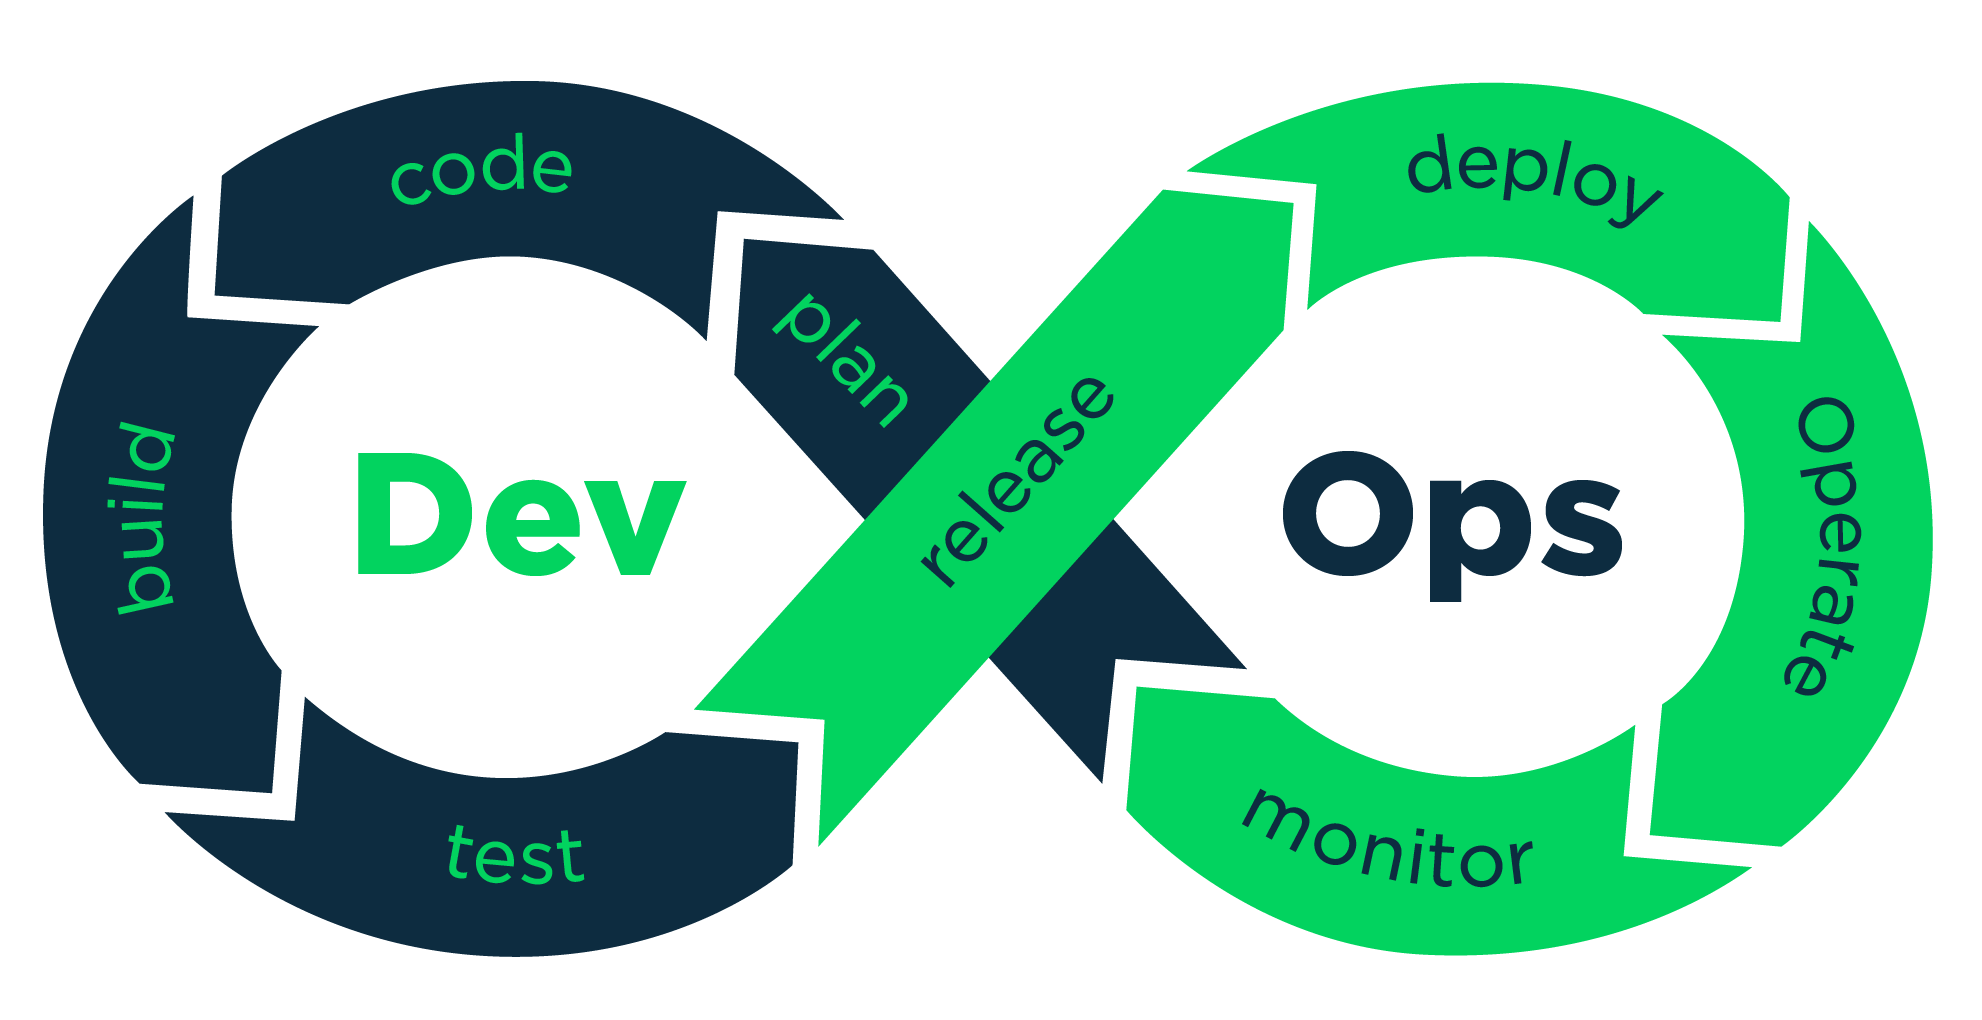
\includegraphics[width=100mm, keepaspectratio]{figures/devops.png}
    \caption{DevOps szemlélet a projektben}
    \label{fig:devops}
\end{figure}
%-----------------------------------------------------------------------------



% Mellékletek
%\input{content/survey}
% Ábrák listája - a word-ös sablon szerint szükséges
%~~~~~~~~~~~~~~~~~~~~~~~~~~~~~~~~~~~~~~~~~~~~~~~~~~~~~~~~~~~~~~~~~~~~~~~~~~~~~~~~~~~~~~
\listoffigures\addcontentsline{toc}{chapter}{\listfigurename}

% Táblázatok listája - opcionális
%~~~~~~~~~~~~~~~~~~~~~~~~~~~~~~~~~~~~~~~~~~~~~~~~~~~~~~~~~~~~~~~~~~~~~~~~~~~~~~~~~~~~~~
%\listoftables\addcontentsline{toc}{chapter}{\listtablename}

% Irodalomjegyzék
%~~~~~~~~~~~~~~~~~~~~~~~~~~~~~~~~~~~~~~~~~~~~~~~~~~~~~~~~~~~~~~~~~~~~~~~~~~~~~~~~~~~~~~
\addcontentsline{toc}{chapter}{\bibname}
\bibliography{bib/references}

% Függelékek
%~~~~~~~~~~~~~~~~~~~~~~~~~~~~~~~~~~~~~~~~~~~~~~~~~~~~~~~~~~~~~~~~~~~~~~~~~~~~~~~~~~~~~~
%%----------------------------------------------------------------------------
\appendix
%----------------------------------------------------------------------------
\chapter*{\fuggelek}\addcontentsline{toc}{chapter}{\fuggelek}
\setcounter{chapter}{\appendixnumber}
%\setcounter{equation}{0} % a fofejezet-szamlalo az angol ABC 6. betuje (F) lesz
\numberwithin{equation}{section}
\numberwithin{figure}{section}
\numberwithin{lstlisting}{section}
%\numberwithin{tabular}{section}

%\label{page:last}
}
\end{document}